\documentclass[final]{beamer}
\usepackage[orientation=landscape,size=custom,width=121.92,height=91.44,scale=1.06]{beamerposter}
\usetheme{default}
\usefonttheme{serif}
\usepackage{mathptmx}
\usepackage{graphicx}
\usepackage{booktabs}
\usepackage{amsmath,amssymb}
\usepackage{xcolor}
\usepackage{array}
\usepackage{ragged2e}

\definecolor{nyuviolet}{RGB}{87,6,140}
\definecolor{nyuvioletd}{RGB}{57,10,95}
\definecolor{inkgray}{RGB}{45,45,45}
\definecolor{uwgray}{RGB}{90,90,95}

\setbeamertemplate{navigation symbols}{}
\setbeamertemplate{blocks}[rounded][shadow=false]
\setbeamercolor{block title}{bg=nyuviolet,fg=white}
\setbeamercolor{block body}{bg=white,fg=black}
\setbeamerfont{block title}{series=\bfseries,size=\large}
\setbeamerfont{block body}{size=\normalsize}
\setbeamersize{text margin left=1.4cm,text margin right=1.4cm}

\newcommand{\fcap}[1]{\par\vspace{1.5mm}{\small\itshape #1}}
\newcommand{\hl}[1]{\textbf{\color{nyuvioletd}#1}}
\newcommand{\colh}{70cm}

\begin{document}
\begin{frame}[t]

%================= HEADER =================
\begin{columns}[c]
\begin{column}{0.18\paperwidth}
  \centering
  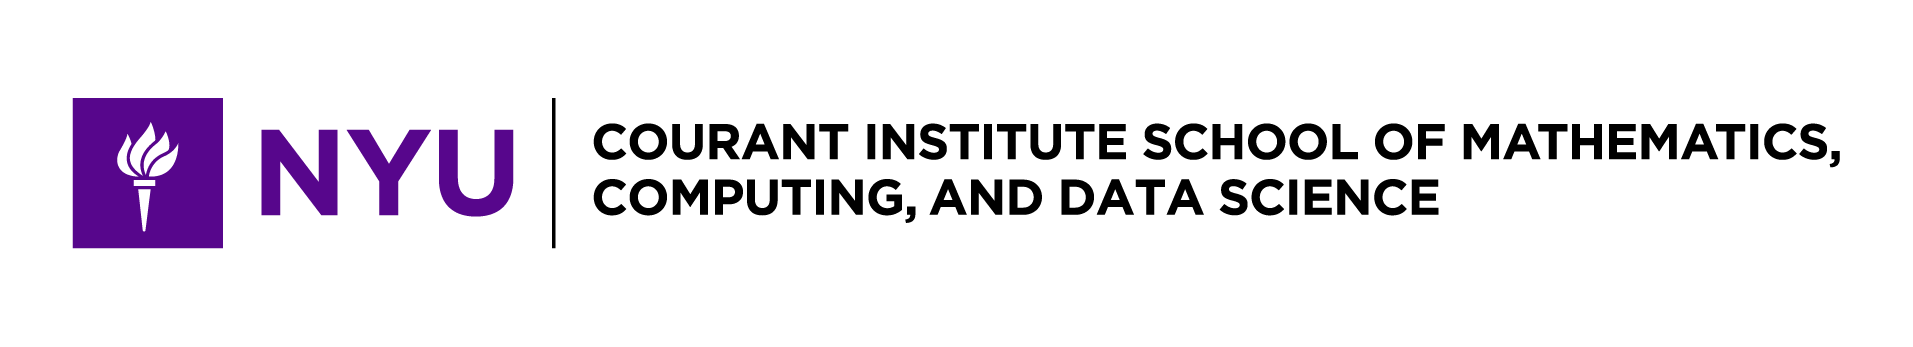
\includegraphics[width=\linewidth]{figs/nyu_logo.png}
\end{column}
\begin{column}{0.62\paperwidth}
  \centering
  {\color{nyuvioletd}\bfseries\fontsize{50}{58}\selectfont A Parameter-Space Study of Stellarator Coil Complexity Across Coil Types}\\[0.4em]
  {\color{inkgray}\fontsize{30}{38}\selectfont \emph{What makes a stellarator hard to coil?}\quad Plasma-shape drivers across 500 quasi-isodynamic equilibria}\\[0.6em]
  {\fontsize{30}{36}\selectfont Logan Tsai\textsuperscript{1}\quad Lanke Fu\textsuperscript{1}\quad Alan A. Kaptanoglu\textsuperscript{2}}\\[0.3em]
  {\normalsize \textsuperscript{1}Courant Institute of Mathematical Sciences, New York University \qquad \textsuperscript{2}W. E. Boeing Dept.\ of Aeronautics \& Astronautics, University of Washington}\\[0.3em]
  {\itshape 68th APS DPP Conference, Chicago, IL, November 2--6, 2026 \quad$\cdot$\quad Poster 48 (BP11)}
\end{column}
\begin{column}{0.18\paperwidth}
  \centering
  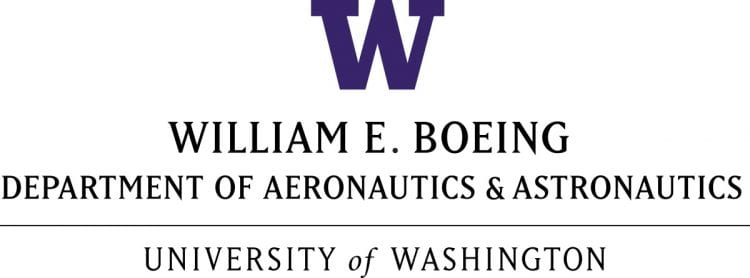
\includegraphics[width=0.62\linewidth]{figs/uw_logo.png}
\end{column}
\end{columns}
\vspace{0.4em}
{\color{nyuviolet}\rule{\linewidth}{4pt}}
\vspace{0.8em}

%================= BODY =================
\begin{columns}[t,onlytextwidth]

%------------- COLUMN 1 -------------
\begin{column}{0.315\textwidth}
\begin{minipage}[t][\colh][t]{\linewidth}

\begin{block}{Motivation}
Stellarator confinement is produced by complex 3D coils, and \hl{coil complexity drives cost and feasibility}. A common assumption is that \emph{high rotational transform ($\iota$) devices are hard to coil with dipoles}.
\vspace{0.3em}

With a large dataset we can test this directly: \hl{which plasma-shape features actually make the coils hard to build?}
\end{block}

\vfill

\begin{block}{The scan}
We run the \hl{quadcoil} winding-surface optimizer over ${\sim}500$ quasi-isodynamic (QI, $N_{fp}=3$) equilibria from the \hl{ConStellaration} dataset. A current potential $\Phi$ on a winding surface sets the sheet current $\mathbf{K}=\mathbf{n}\times\nabla\Phi$; we solve for the field that reproduces the plasma boundary and read off a coil \emph{cost} at a fixed field-error budget:
\vspace{0.2em}
\begin{equation*}
f_B=\frac{\oint (\mathbf{B}\cdot\mathbf{n})^2\,dA}{\oint |\mathbf{B}|^2\,dA},
\qquad \text{feasible}: f_B\le 1.01\,f_B^{\text{target}}.
\end{equation*}
Six coil problems per configuration; \emph{cost} is the objective achieved at the budget:
\vspace{0.4em}

\centering
\renewcommand{\arraystretch}{1.35}
\begin{tabular}{@{}lll@{}}
\toprule
\textbf{Problem} & \textbf{Objective} & \textbf{Penalizes}\\
\midrule
sparse dipole & $f_{\ell_1\Phi}$ & dipole count ($\ell_1$)\\
thin dipole & $f_{\max\Phi}$ & peak current ($\ell_\infty$)\\
min-force dipole & $f_{\max F}$ & peak coil force\\
low-curv filament & $f_{\max\kappa}$ & filament curvature\\
min-force filament & $f_{\max F}$ & peak coil force\\
L2 current pot.\ & $f_{\Phi}$ & smooth current ($\ell_2$)\\
\bottomrule
\end{tabular}
\end{block}

\vfill

\begin{block}{Coils from a current potential}
\centering
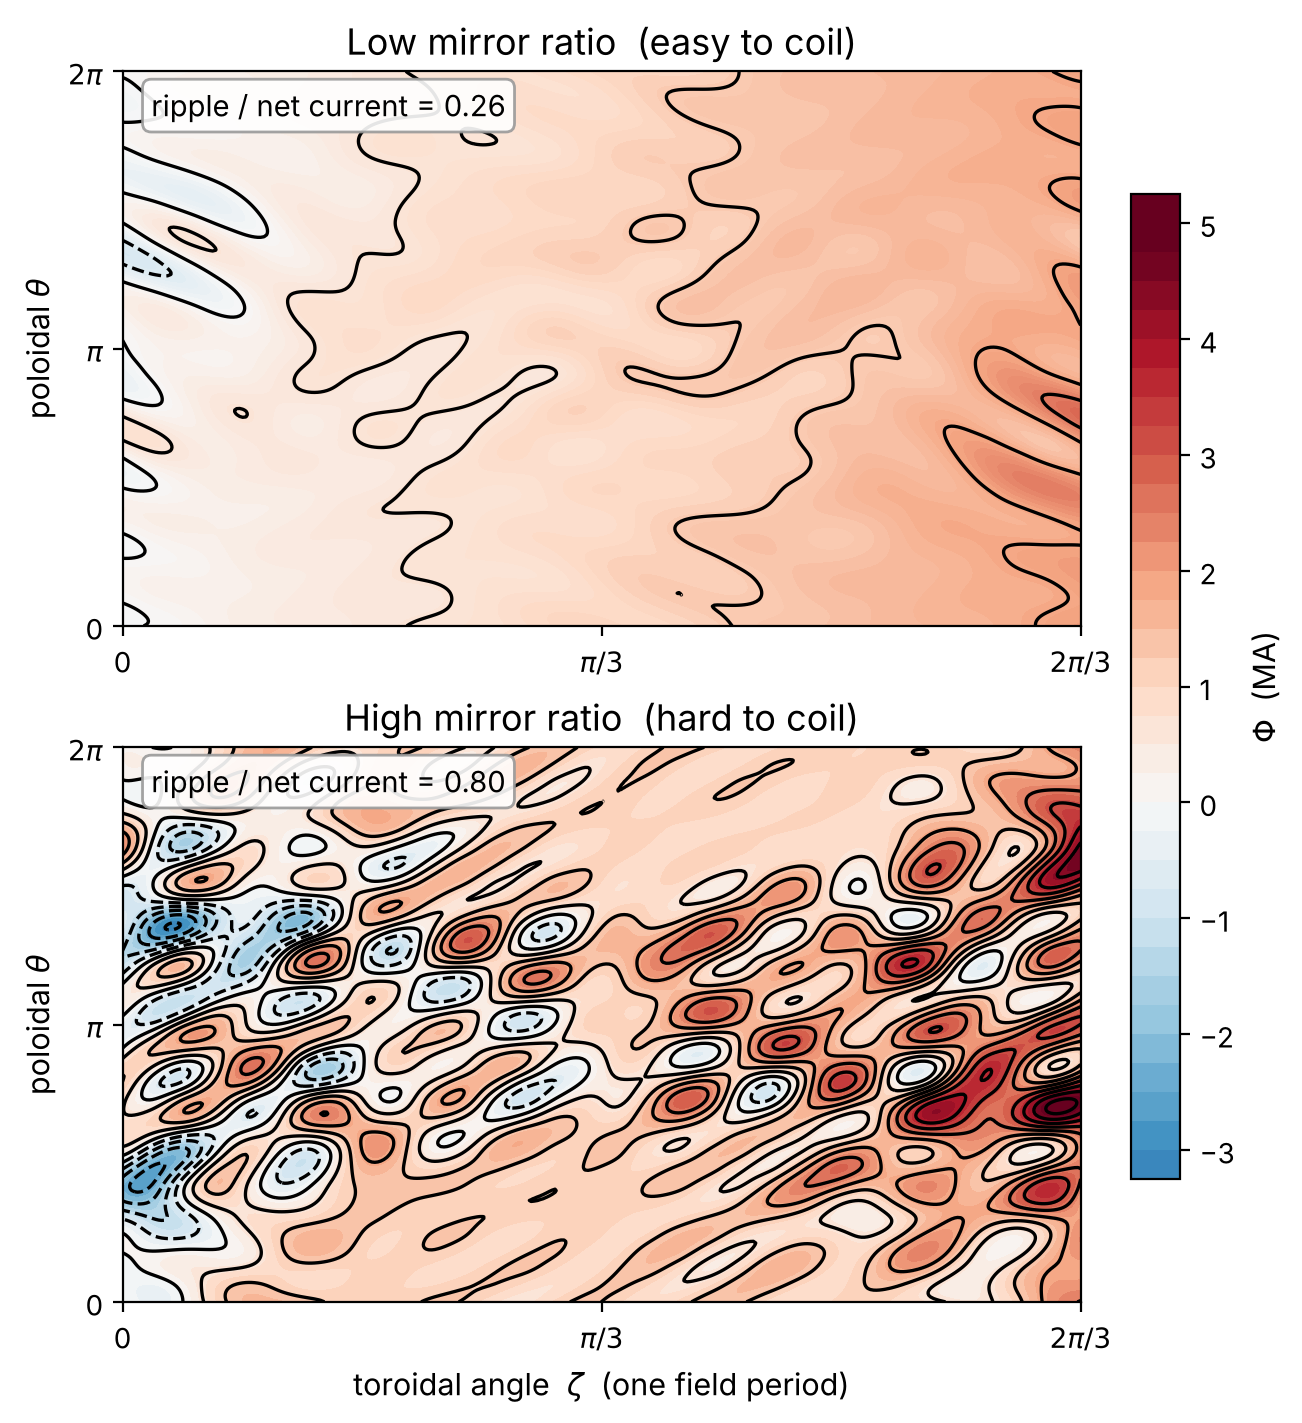
\includegraphics[width=0.94\linewidth]{figs/phi_compare_v.png}
\fcap{Current potential $\Phi$ on the winding surface, one field period; \hl{the black lines are the coils} (contours of $\Phi$). The low-mirror case needs a few smooth coils; the high-mirror case needs many more, and they are contorted with closed windowpane islands. The single-valued ripple relative to the net current rises from $0.26$ to $0.80$.}
\end{block}

\end{minipage}
\end{column}

%------------- COLUMN 2 -------------
\begin{column}{0.315\textwidth}
\begin{minipage}[t][\colh][t]{\linewidth}

\begin{block}{What drives coil complexity?}
\centering
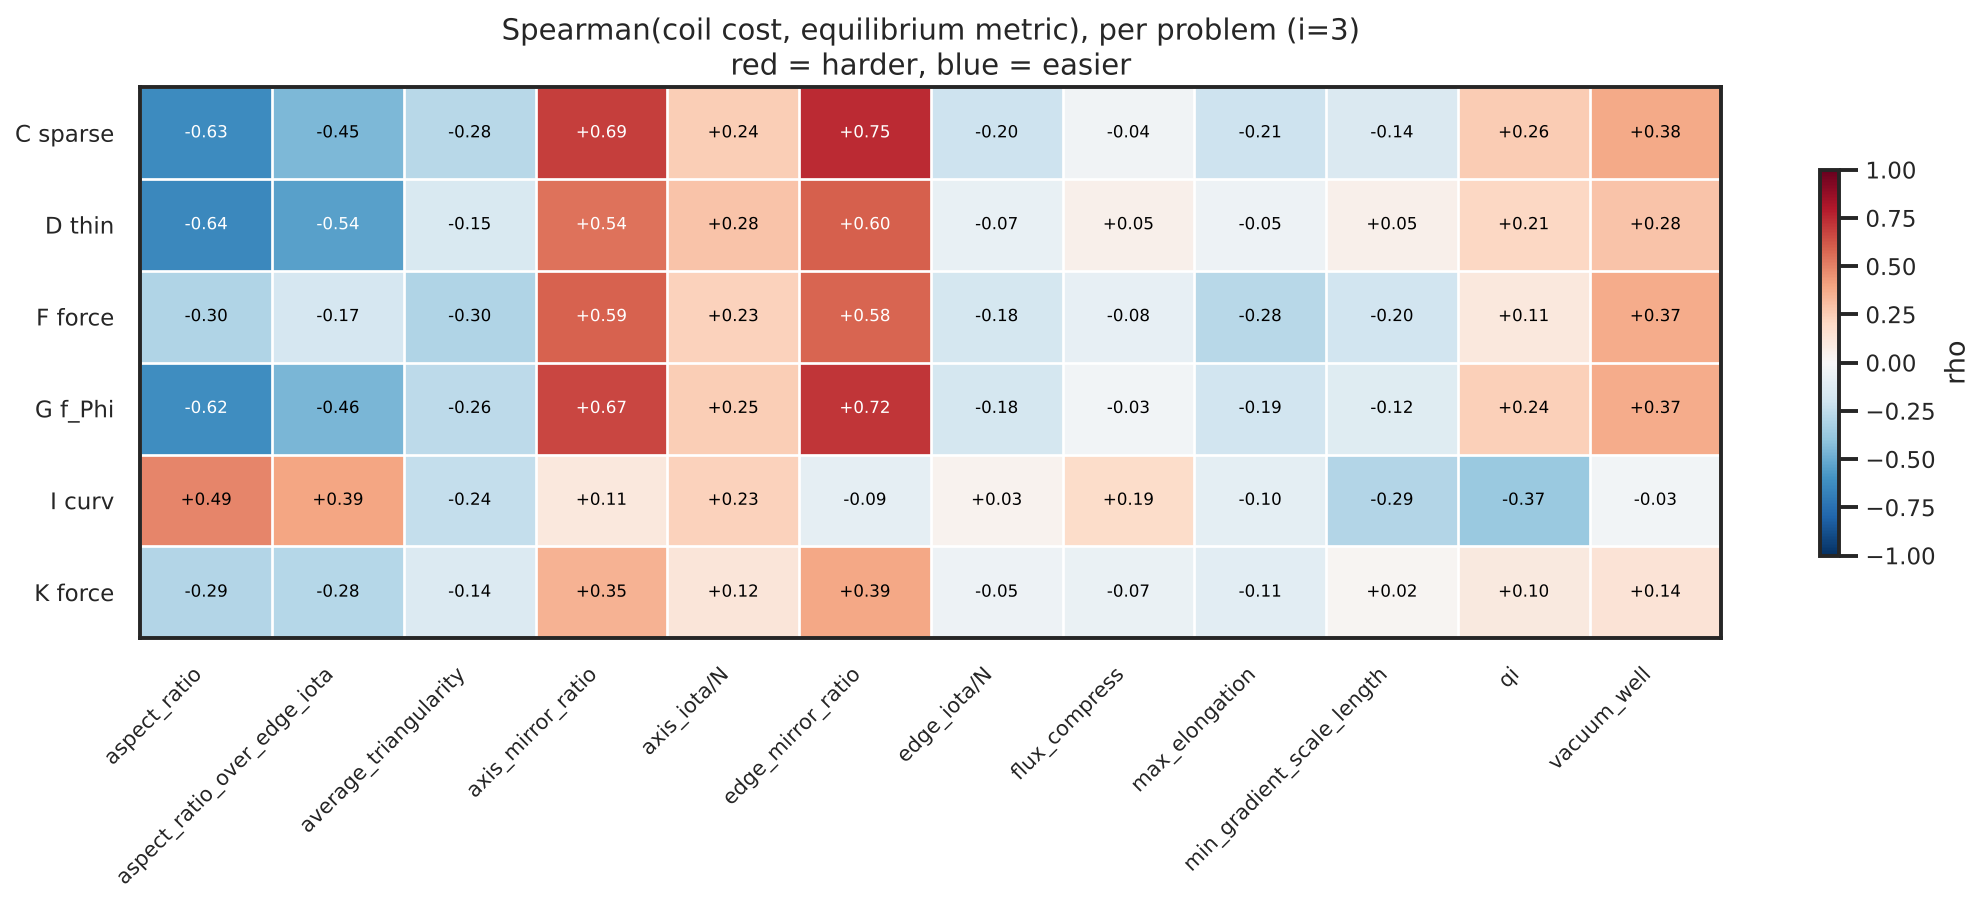
\includegraphics[width=\linewidth]{figs/metric_colormap.png}
\fcap{Spearman $\rho$ of coil cost vs each ConStellaration metric, per problem (red = harder, blue = easier). \hl{Mirror ratio} (axis \& edge) and \hl{aspect ratio} are the strong, consistent signals; the two $\iota$ columns are weak and opposite in sign.}
\end{block}

\vfill

\begin{block}{Mirror ratio, not rotational transform}
\centering
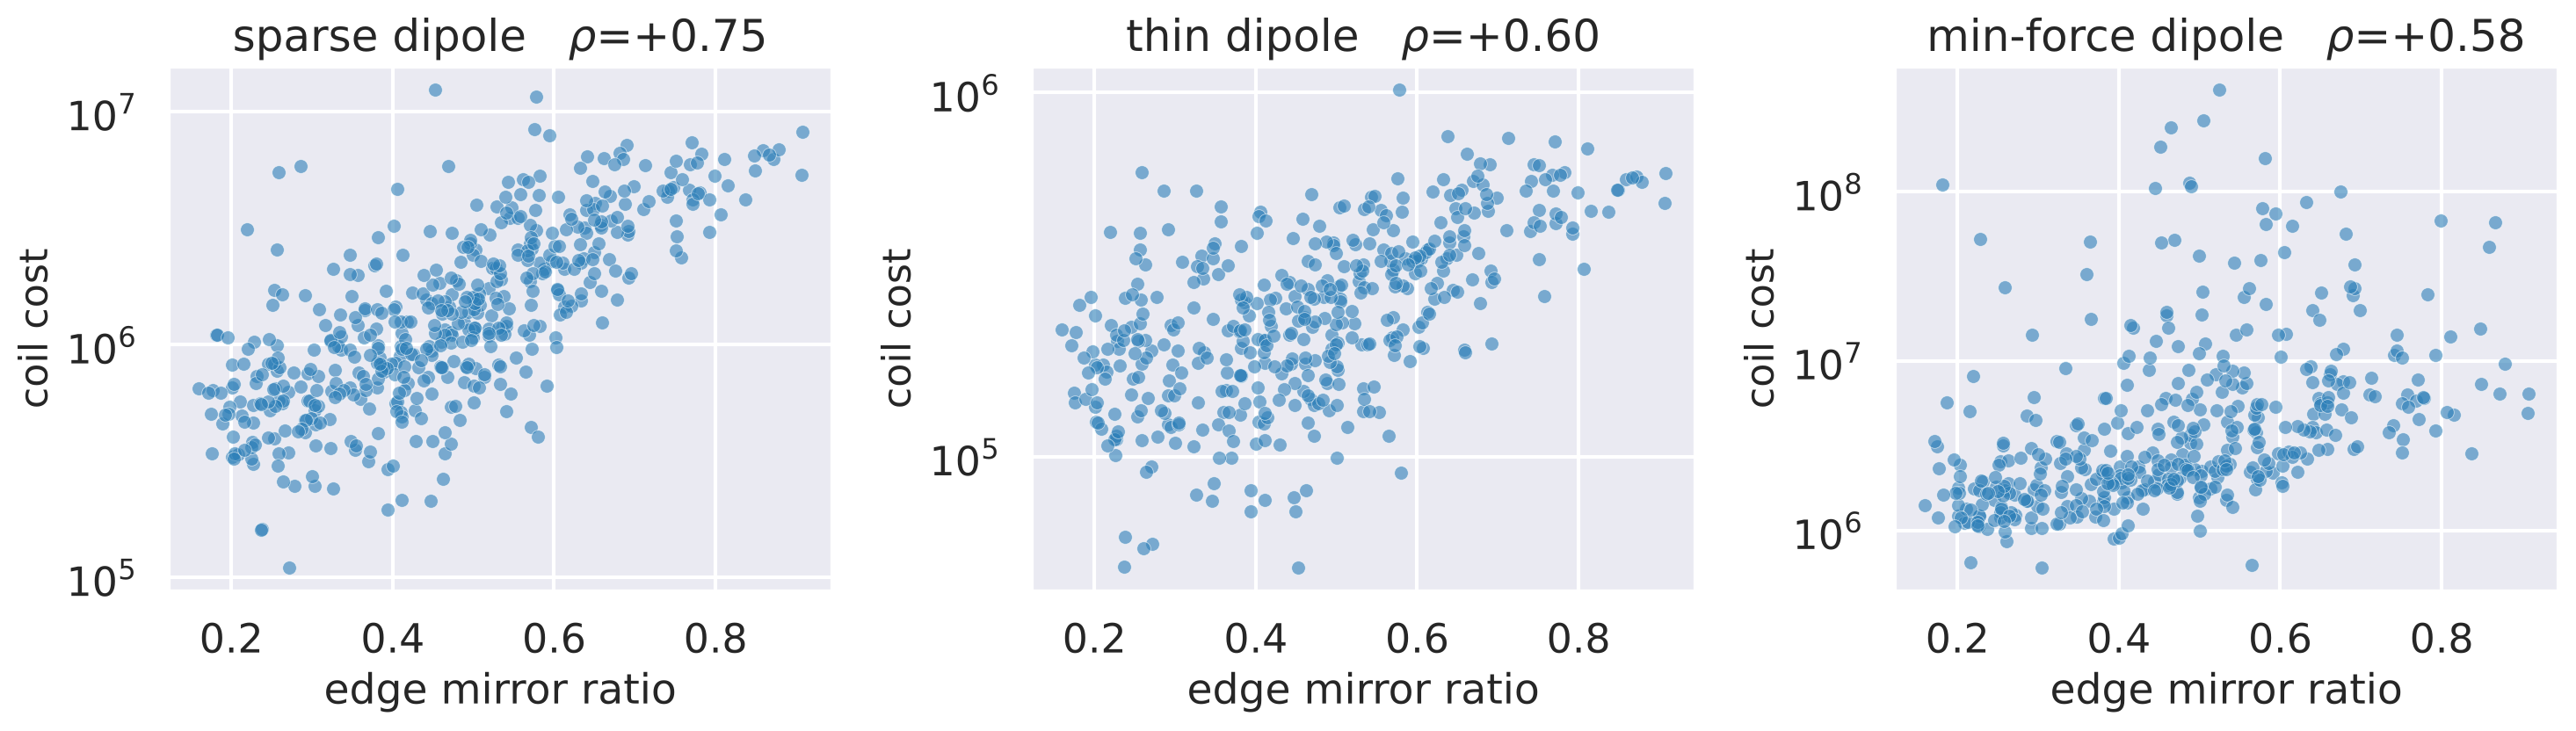
\includegraphics[width=0.92\linewidth]{figs/mirror_row.png}\\[0.5em]
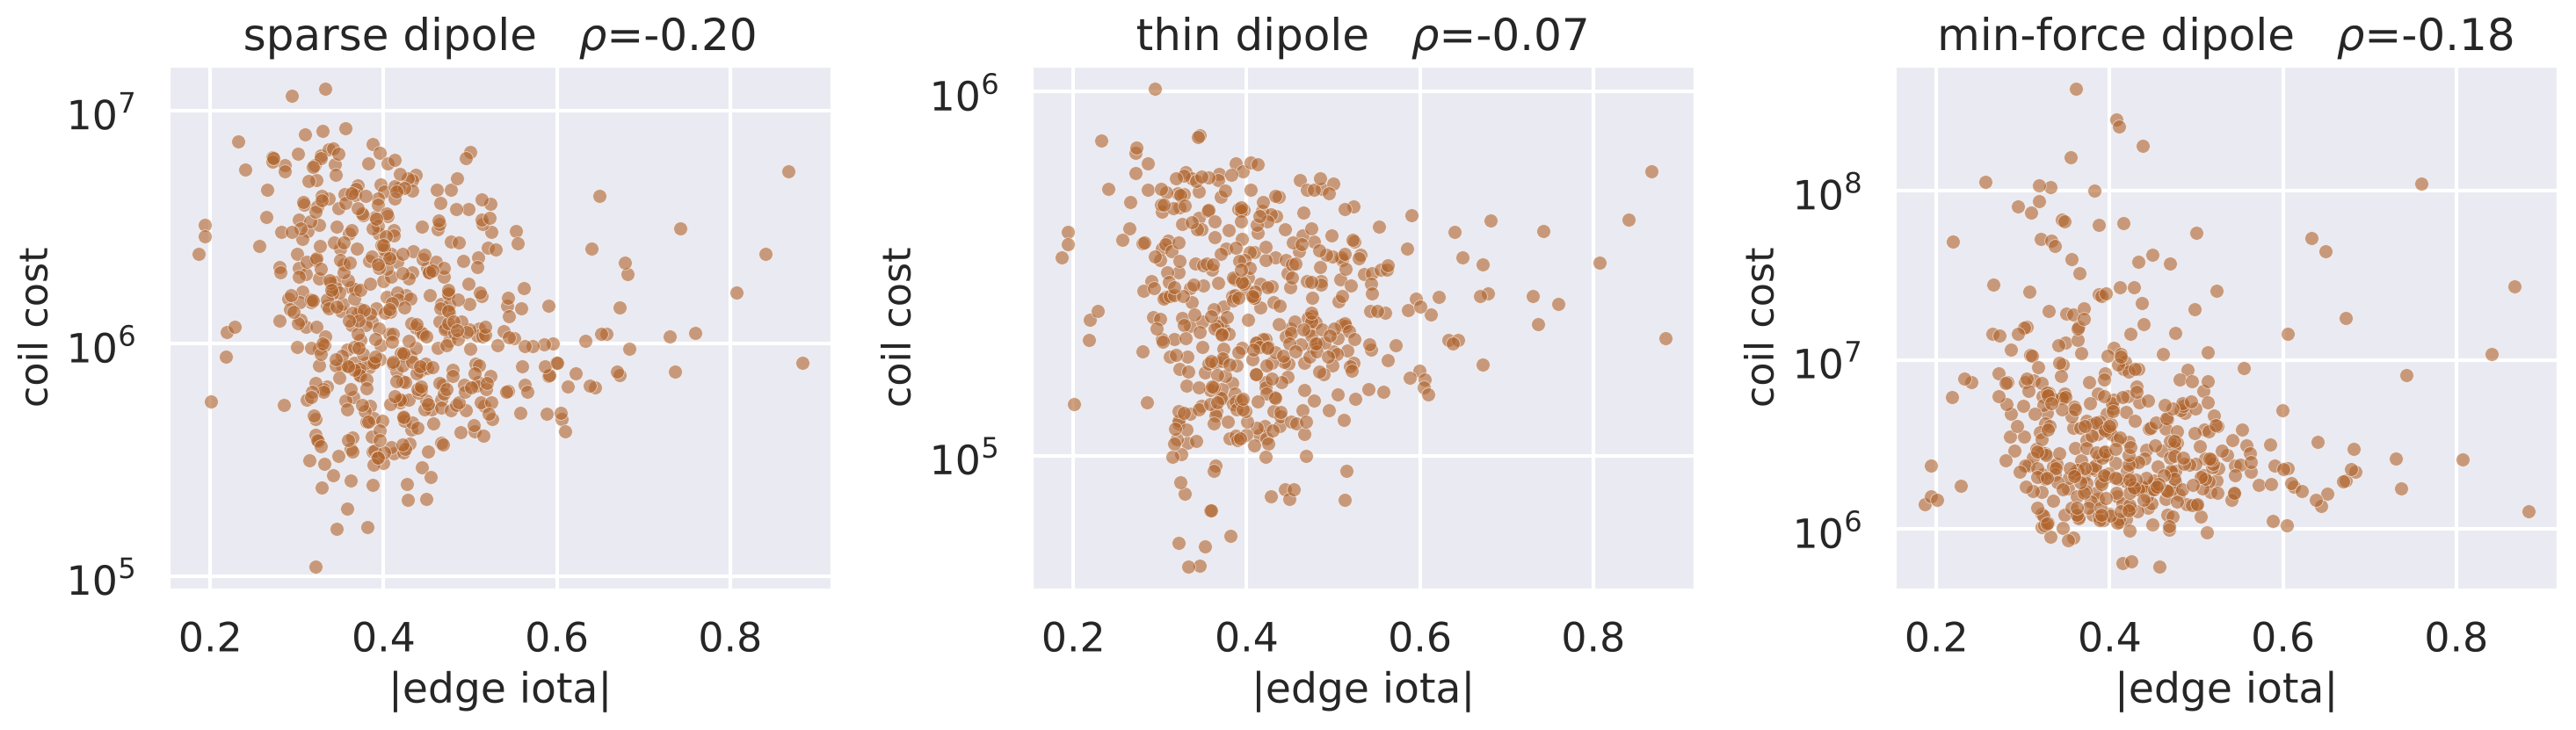
\includegraphics[width=0.92\linewidth]{figs/iota_row.png}
\fcap{Dipole cost rises steeply with mirror ratio ($\rho=+0.58$ to $+0.75$, top) but shows no clear trend with rotational transform (bottom), contrary to the common assumption.}
\end{block}

\vfill

\begin{block}{Is it causal, or just collinearity?}
Plasma parameters are correlated among themselves, so a raw correlation can over-credit a correlated variable. The \hl{coefficient of multiple correlation} isolates each feature's unique contribution: \ $R=\sqrt{\mathbf{c}^{\top}\mathbf{R}^{-1}\mathbf{c}}$, \ weights $\boldsymbol{\beta}=\mathbf{R}^{-1}\mathbf{c}$ \ ($\mathbf{c}$: cost--parameter correlations; $\mathbf{R}$: correlations \emph{among} parameters).
\vspace{0.4em}

\centering
\begin{minipage}{0.52\linewidth}\centering
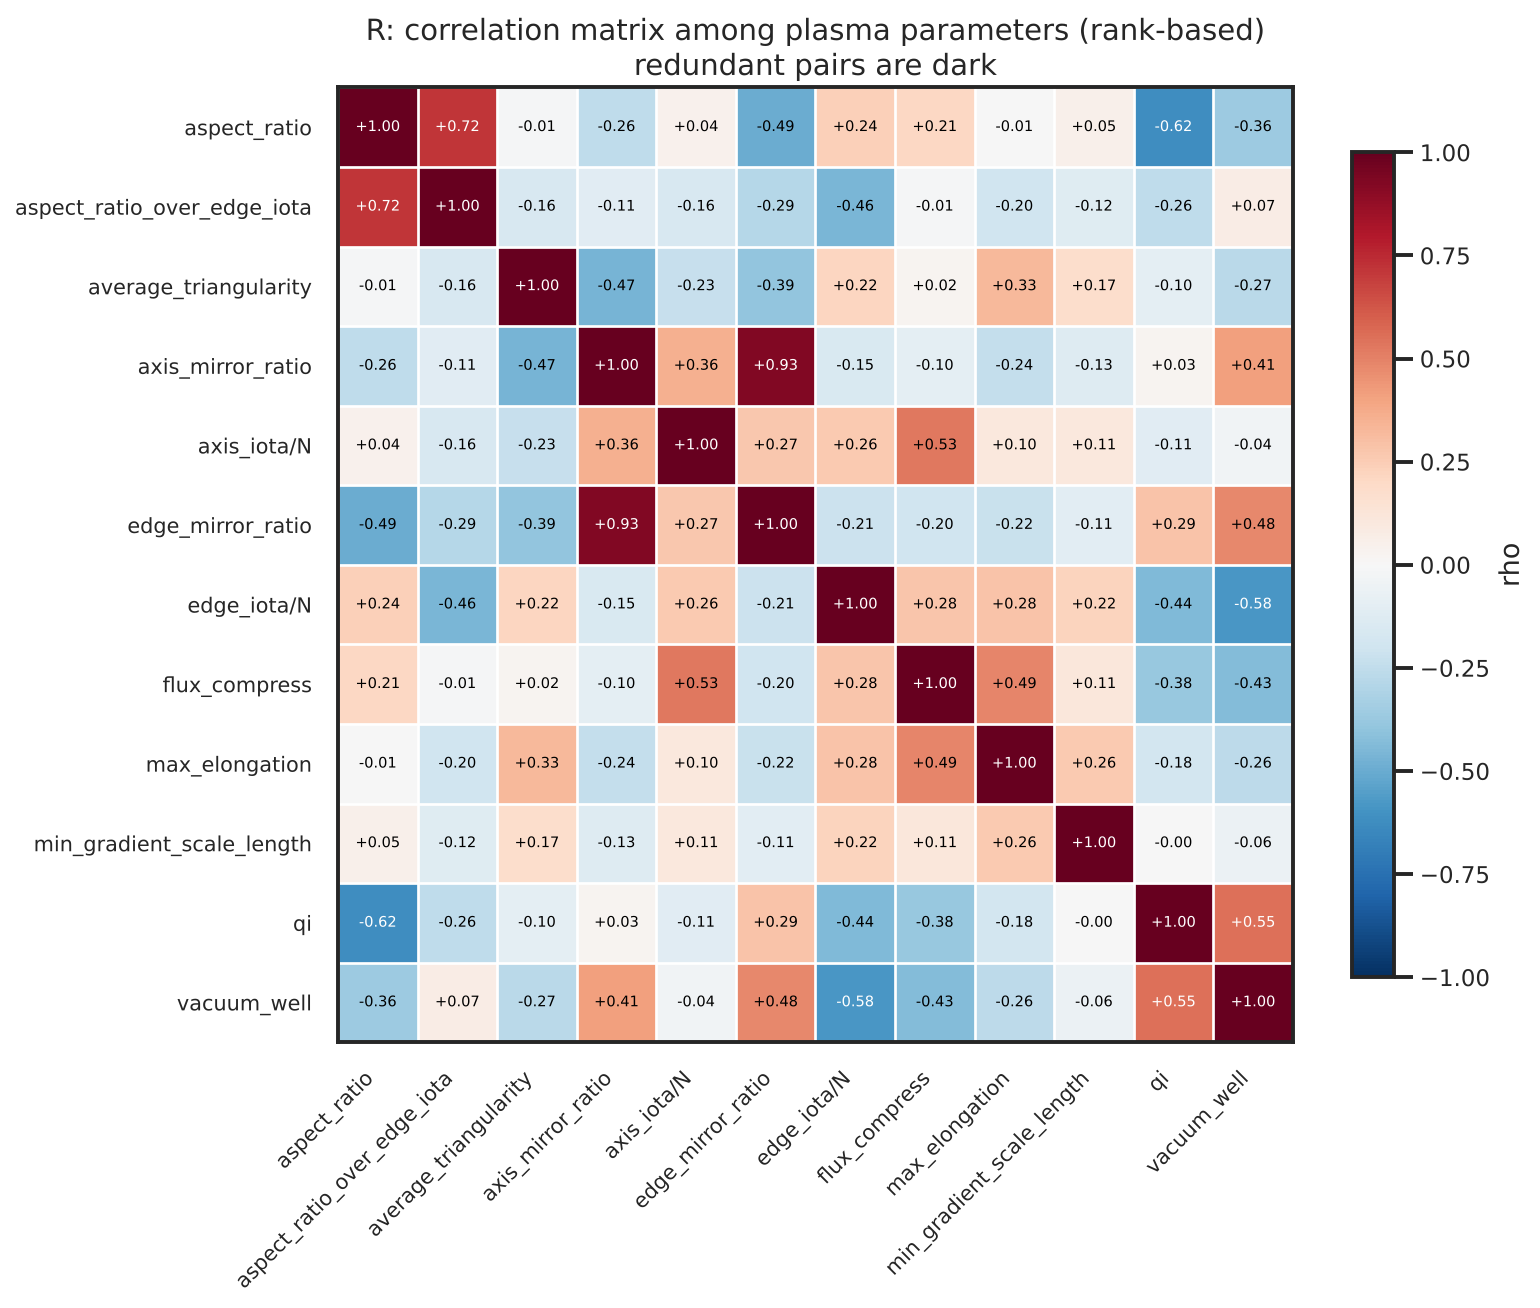
\includegraphics[width=\linewidth]{figs/plasma_corr_matrix.png}
\end{minipage}\hfill
\begin{minipage}{0.46\linewidth}\centering
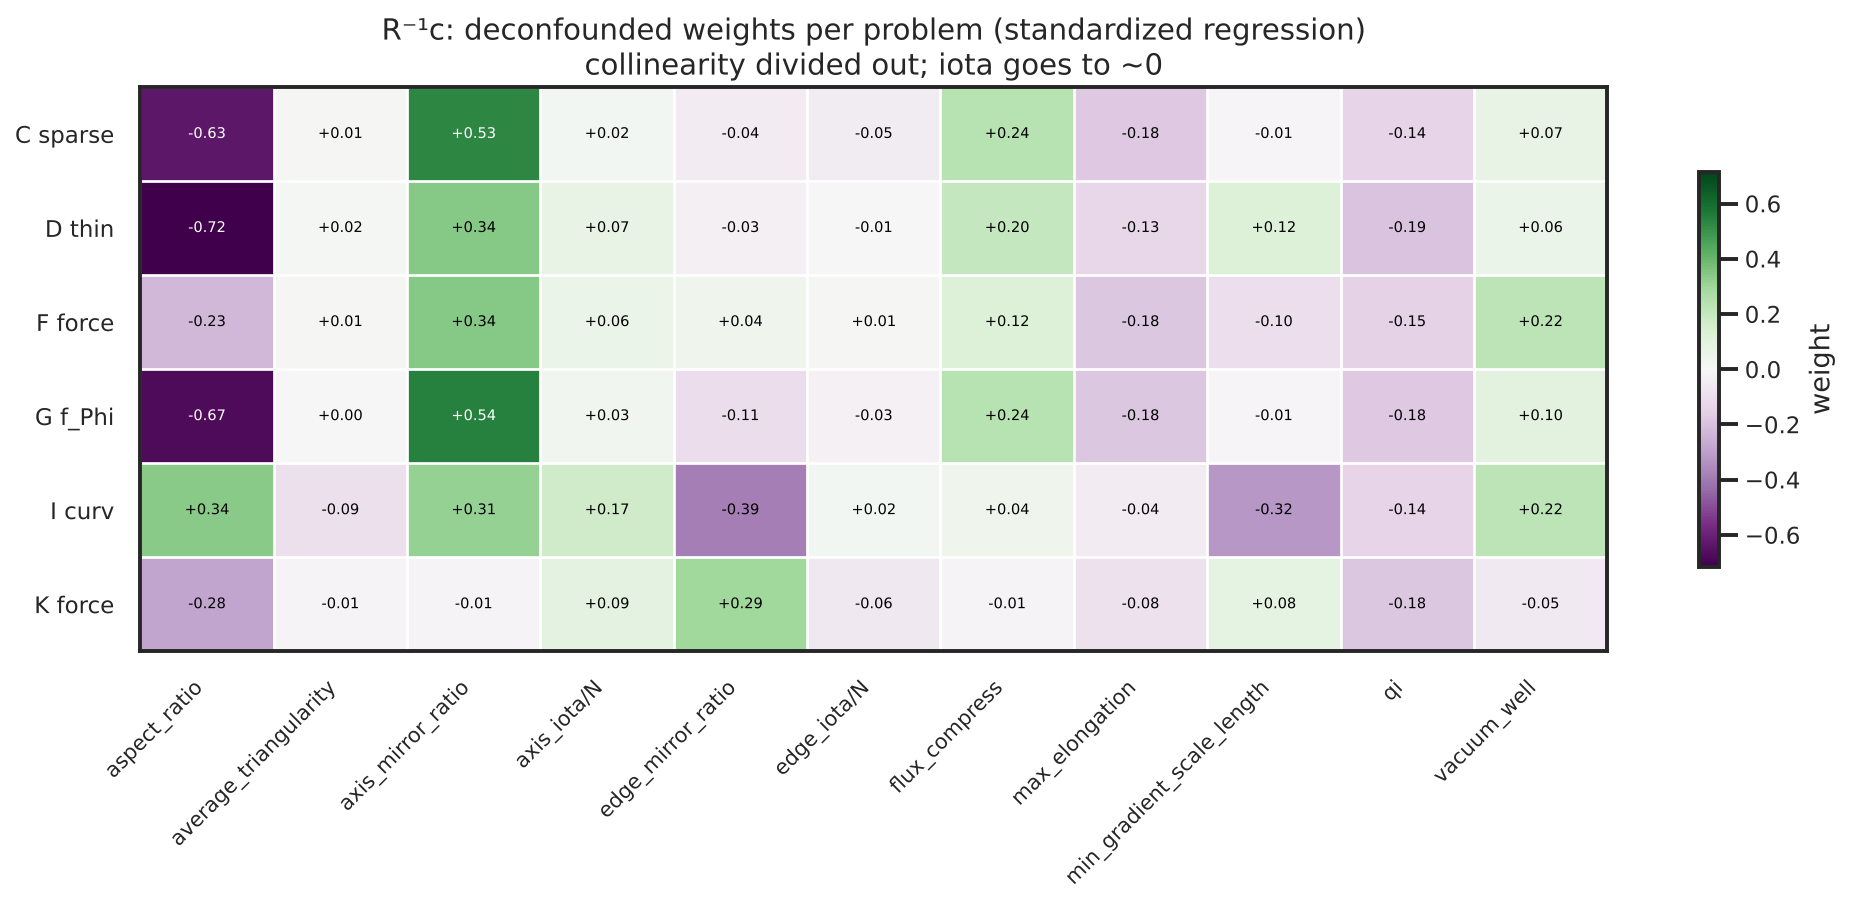
\includegraphics[width=\linewidth]{figs/deconfounded_weights.png}
\end{minipage}
\fcap{Left: parameters are collinear (edge/axis mirror $+0.93$). Right: with collinearity divided out, \hl{aspect ratio and axis mirror ratio remain}, while the $\iota$ weight collapses to ${\approx}0$. The driver is field-strength modulation and compactness, not rotational transform.}
\end{block}

\end{minipage}
\end{column}

%------------- COLUMN 3 -------------
\begin{column}{0.315\textwidth}
\begin{minipage}[t][\colh][t]{\linewidth}

\begin{block}{$f_{\Phi}$: a cheap, well-conditioned proxy}
\centering
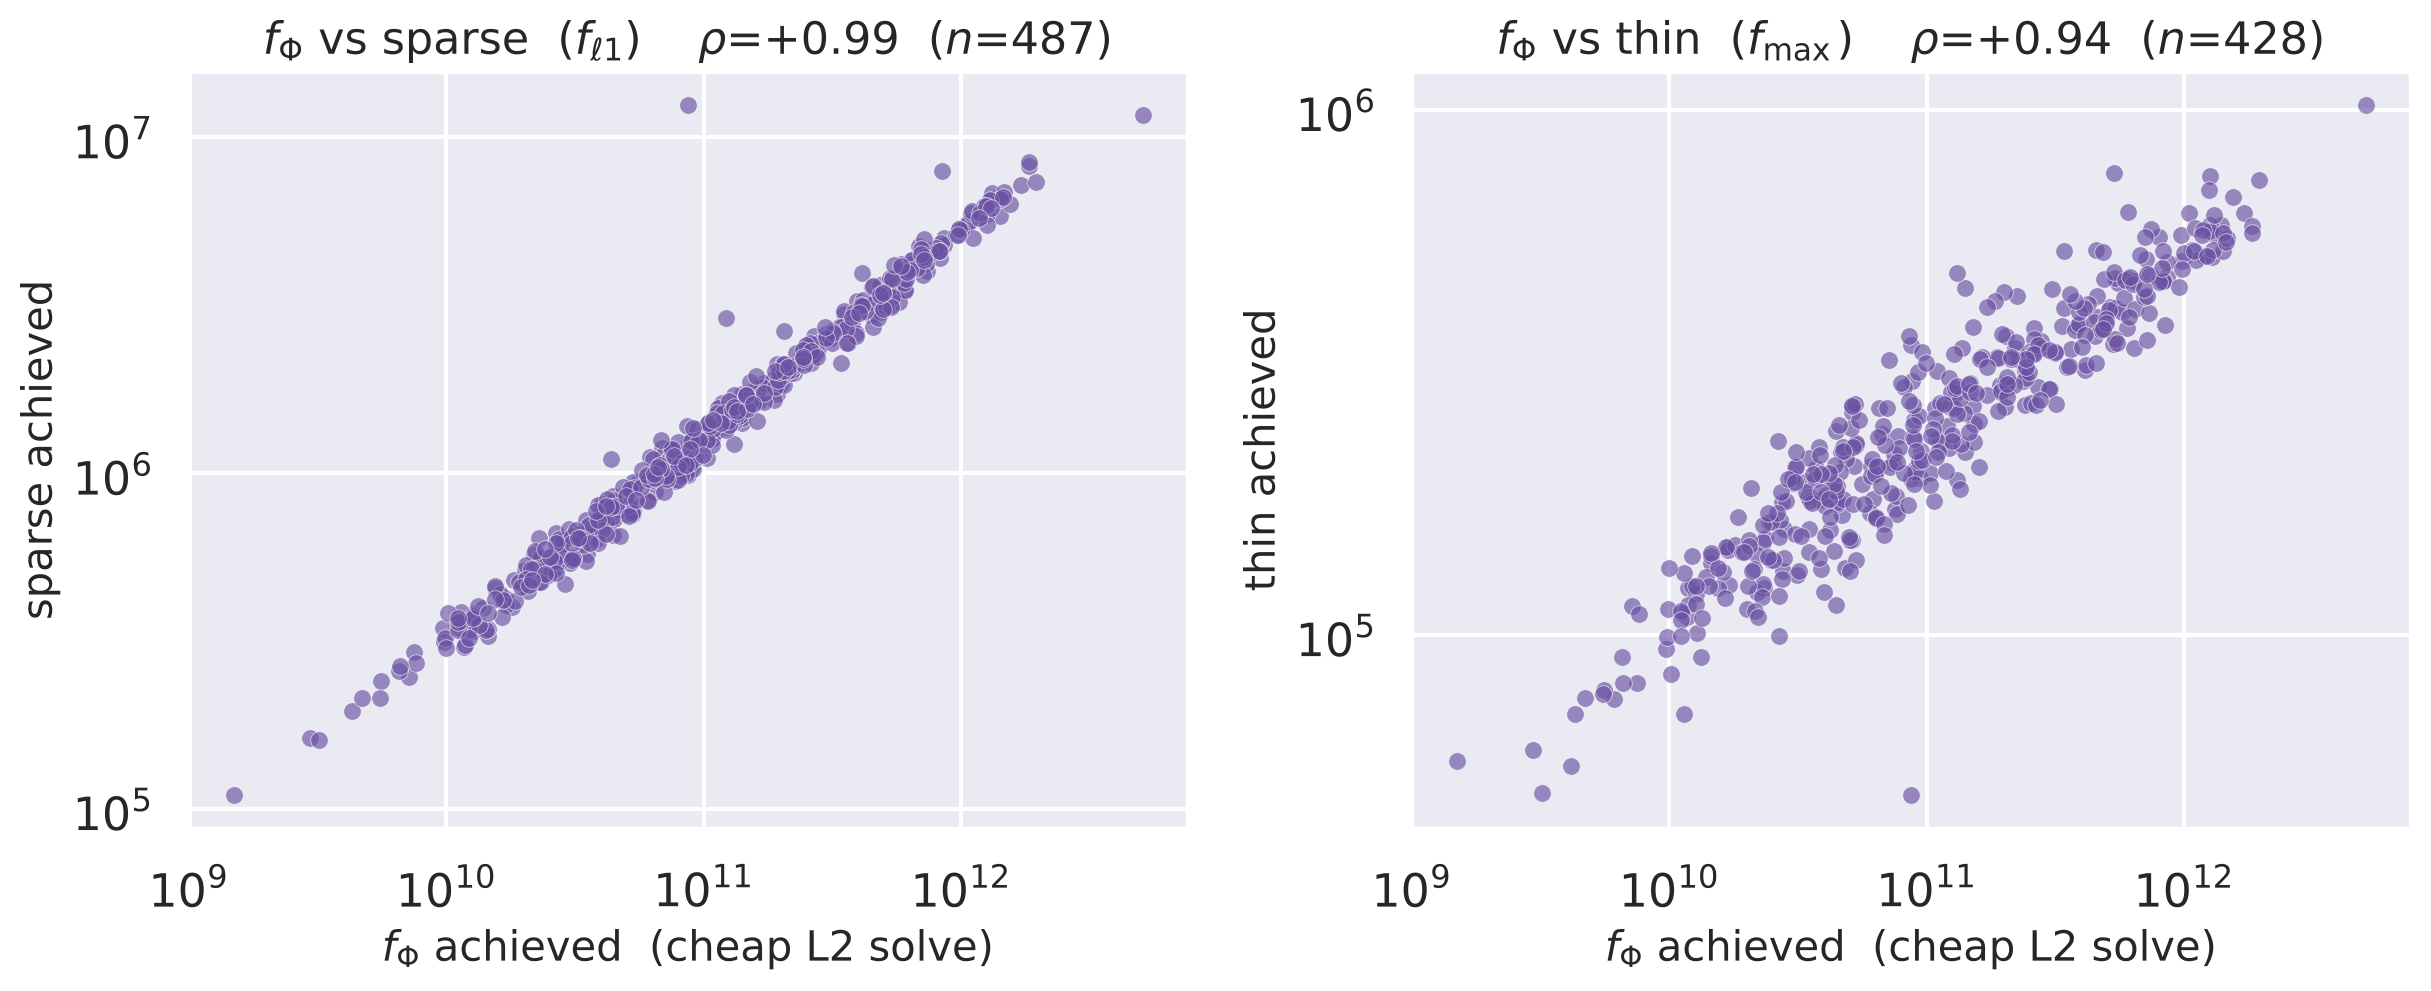
\includegraphics[width=\linewidth]{figs/fphi_correlation.png}
\fcap{$f_{\Phi}$ (cheap L2 solve) vs the sparse and thin dipole costs; $n=487$ and $428$ (full ${\sim}500$ sweep).}
\justifying
\vspace{0.4em}
\begin{itemize}\setlength{\itemsep}{0.35em}
\item A single well-conditioned linear solve.
\item Tracks sparse / thin dipole cost: $\rho=+0.99 / +0.94$.
\item Smooth quadratic (good Hessian); $\ell_1/\ell_\infty$ are smoothed but nearly flat, so Newton struggles.
\item A cheap \hl{difficulty screen} and candidate coil term for single-stage optimization.
\end{itemize}
\end{block}

\vfill

\begin{block}{Findings}
\begin{itemize}\setlength{\itemsep}{0.3em}
\item Mirror ratio and aspect ratio predict dipole coil complexity, \hl{not rotational transform}.
\item $f_{\Phi}$ is a cheap, well-conditioned proxy for the dipole-complexity objectives.
\end{itemize}
\vspace{0.3em}
\textbf{Scope.}\ \ QI $N_{fp}{=}3$, current-potential formulation, one fixed $f_B$ budget; these are associations (deconfounding controls measured metrics only).
\end{block}

\vfill

\begin{block}{The current potential in 3D}
\centering
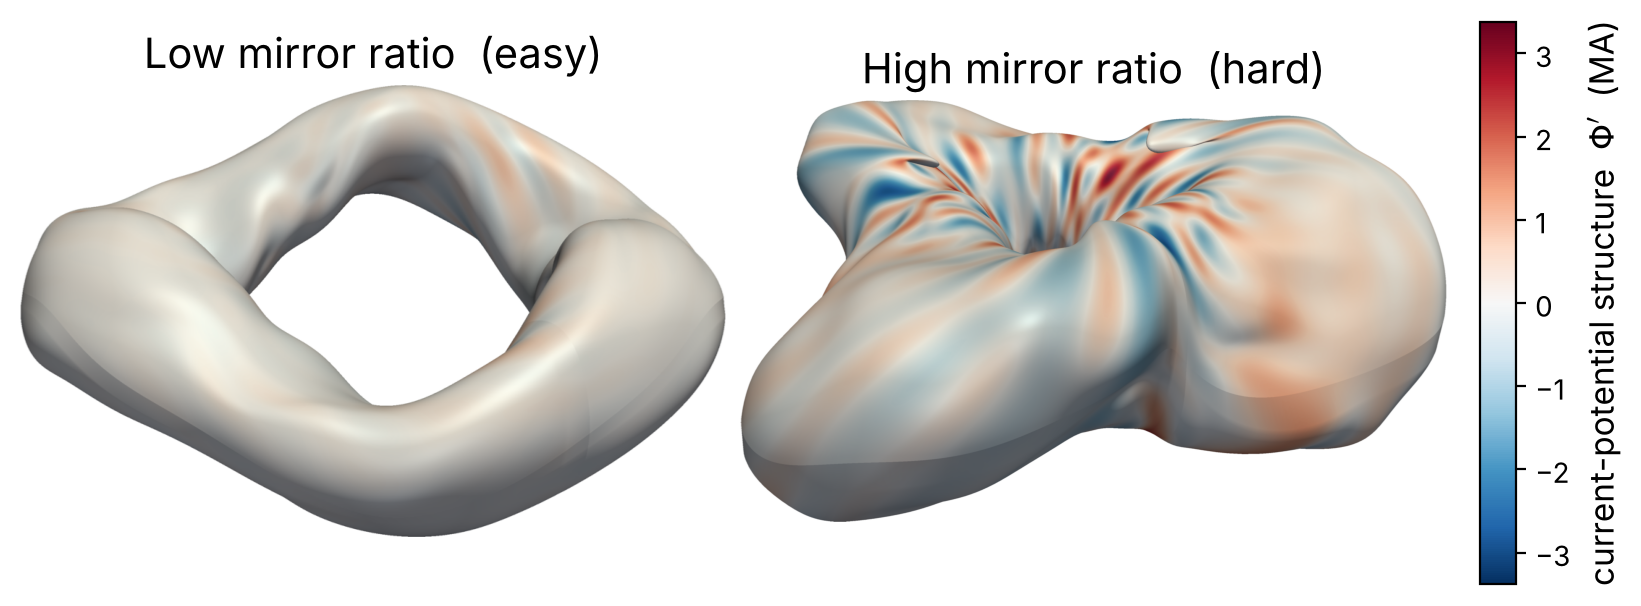
\includegraphics[width=0.96\linewidth]{figs/surface_compare_v.png}
\fcap{Current-potential structure $\Phi'$ painted on the two winding surfaces (single-valued part, same scale). Low mirror ratio: smooth and nearly uniform, so the coils stay simple. High mirror ratio: strongly structured, so the coils become complex.}
\end{block}

\vfill

\begin{block}{Next steps}
\begin{itemize}\setlength{\itemsep}{0.35em}
\item Confirm the $f_{\Phi}$ proxy across all $f_B$ budgets (shown here at one budget, now on the full ${\sim}500$).
\item Fold $f_{\Phi}$ into single-stage (plasma $+$ coil) optimization as a cheap, differentiable coil term.
\item Pin down the mechanism: \emph{why} mirror ratio sets the required sheet-current structure.
\item Extend beyond QI $N_{fp}{=}3$ (QA, QH, other field periods): does mirror $+$ aspect generalize?
\item Carry the drivers to cut filamentary coils with engineering limits (distance, HTS length); model \emph{feasibility}, not just cost.
\end{itemize}
\end{block}

\vfill

\begin{block}{References \& contact}
\begin{minipage}[c]{0.82\linewidth}
{\small
QUADCOIL: Fu \textit{et al.} \ $\cdot$\ REGCOIL: Landreman \& Boozer. \ $\cdot$\ ConStellaration: Proxima Fusion (HuggingFace).\\[0.3em]
Contact: \texttt{lct9592@nyu.edu} \ $\cdot$\ Kaptanoglu group, Courant Institute (NYU).\\[0.3em]
Code: \texttt{github.com/logantsai07/ConstellarationProject}}
\end{minipage}\hfill
\begin{minipage}[c]{0.15\linewidth}\centering
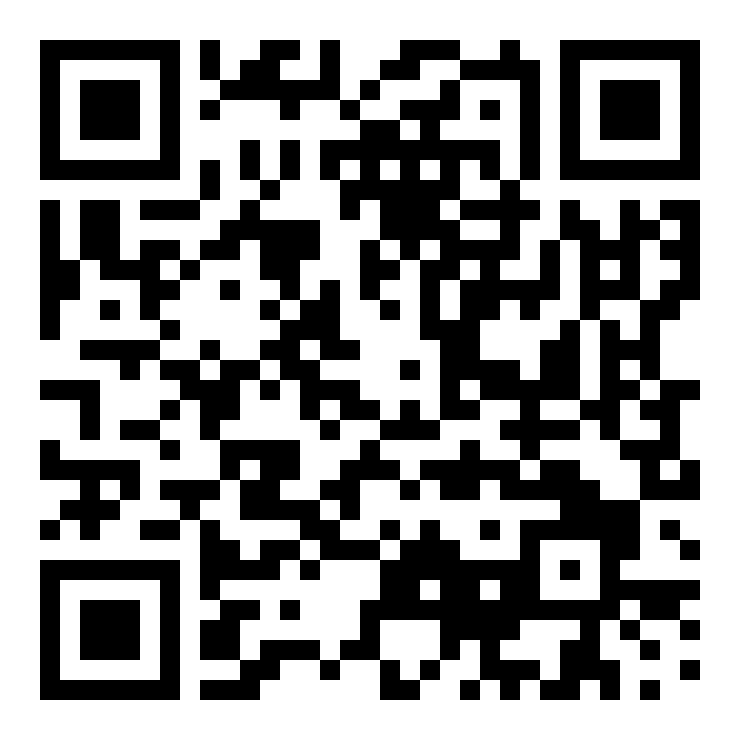
\includegraphics[width=\linewidth]{figs/qr.png}\\[0.1em]
{\scriptsize scan for code}
\end{minipage}
\end{block}

\end{minipage}
\end{column}
\end{columns}
\end{frame}
\end{document}
